\chapter{Rashba force in the Thiele equation}\label{app:F_RashbaThiele}
The Rashba force in the Thiele equation is given by
\begin{align}
    \mathbold{F}_{\text{R}} = -\mu_0\int\d V\sum_k(\mathbold{\nabla}M_k)\left(\mathbold{H}_{\text{R}}-\frac{\beta}{M_s}\mathbold{M}\times\mathbold{H}_{\text{R}}\right)_k
\end{align}
with $\mathbold{H}_{\text{R}} = C_{\text{R}} b_J\mathbold{\hat{y}}$ for a broken inversion symmetry in the $z$-direction and an applied current in the $x$-direction. We will first consider the force 
\begin{align}
    \mathbold{F}_{\text{R}}^{(1)} = -\mu_0\int\d V\sum_k(\mathbold{\nabla}M_k)\left(\mathbold{H}_{\text{R}}\right)_k.
\end{align}
To do this we must know $\partial_x m_y$ and $\partial_y m_y$. We note for the remainder of this chapter that $\partial_z \mathbold{M} = 0$. To find these derivatives we use the chain rule and the following relations obtained from the ansatz $\theta = \theta(r)$ and identity $\tan\phi=x/y$:
\begin{subequations}
\begin{align}
    \partial_x\theta &= \cos\phi \partial_r \theta, \\
    \partial_y\theta &= \sin\phi\partial_r\theta, \\
    \partial_x\Phi &= -\frac{\sin\phi}{r}, \\
    \partial_y\Phi &= \frac{\cos\phi}{r}.
\end{align}
\end{subequations}
We then find that
\begin{subequations}
\begin{align}
    \partial_x m_y &= \partial_x(\sin\theta\sin\Phi) = \cos\theta\sin\Phi\cos\phi\partial_r\theta - \frac{\sin\theta}{r}\cos\Phi\sin\phi, \\
    \partial_y m_y &= \partial_y(\sin\theta\sin\Phi) = \cos\theta\sin\Phi\sin\phi\partial_r\theta + \frac{\sin\theta}{r}\cos\Phi\cos\phi.
\end{align}
\end{subequations}
Using these results we end up with the force
\begin{align}
    \mathbold{F}_{\text{R}}^{(1)} = -\mu_0C_{\text{R}}b_J M_s\int\d V
    \begin{pmatrix}
    (\sin\psi+\cos\Phi\sin\phi)\partial_r\theta-\frac{\sin\theta}{r}\cos\Phi\sin\phi \\
    (\cos\psi-\cos\Phi\cos\phi)\partial_r\theta+\frac{\sin\theta}{r}\cos\Phi\cos\phi \\
    0
    \end{pmatrix},
\end{align}
where we have used the relations
\begin{subequations}
\begin{align}
    \sin\Phi\cos\phi-\cos\Phi\sin\phi &= \sin\psi, \\
    \sin\Phi\sin\phi+\cos\Phi\cos\phi &= \cos\psi.
\end{align}
\end{subequations}
In the case of $\psi = 0$ or $\psi=\pi$, we can easily see that two of the components of $\mathbold{F}_{\text{R}}^{(1)}$ are zero, as $\sin\psi=0$ and $\int\d \phi \cos\phi\sin\phi = 0$. The $y$-component can also be seen to be zero. As $\cos\Phi\cos\phi = \cos^2\phi$ and $(\cos\psi-\cos\Phi\cos\phi) = \sin^2\phi$ for $\psi = 0$, $\cos\Phi\cos\phi = -\cos^2\phi$ and $(\cos\psi-\cos\Phi\cos\phi) = -\sin^2\phi$ for $\psi = \pi$, after performing the integral over $\phi$ we remain with a constant times the integral 
\begin{align}
\int_0^{\infty} \d r \left(r\cos\theta\partial_r \theta + \sin\theta\right).
\end{align}
This integral is zero as well, as one can see by performing a partial integration of $\sin\theta(r)$:
\begin{align}
\int_0^{\infty} \d r \sin\theta = r\sin\theta|_{r = 0}^{r=\infty} - \int_0^{\infty} \d r r\cos\theta\partial_r \theta.
\end{align}
Rearranging the terms gives us
\begin{align}
\int_0^{\infty} \d r \left(r\cos\theta\partial_r \theta + \sin\theta\right) = r\sin\theta|_{r = 0}^{r=\infty} = 0.
\end{align}
This integral is zero because $\sin\theta(r)$ decays faster than $1/r$ and is finite at $r=0$, which can be verified numerically. We have then shown that $\mathbold{F}_{\text{R}}^{(1)} = 0$ for $\psi = 0, \pi$. It can be shown in a similar manner that $\mathbold{F}_{\text{R}}^{(1)} = 0$ for $\psi=\pm\pi/2$ as well. We then proceed to consider the second part of the force,
\begin{align}
    \mathbold{F}_{\text{R}}^{(2)} = -\mu_0\int\d V\sum_k(\mathbold{\nabla}M_k)\left(-\frac{\beta}{M_s}\mathbold{M}\times\mathbold{H}_{\text{R}}\right)_k.
    \label{eq:FR2}
\end{align}
The cross-product in the magnetic field can be written out as $-\beta\mathbold{m}\times\mathbold{H}_{\text{R}} = \beta C_{\text{R}} b_J ( \cos\theta \mathbold{\hat{x}} - \sin\theta\cos\Phi\mathbold{\hat{z}} )$. The partial derivatives of $m_x$ and $m_z$ are found to be
\begin{subequations}
\begin{align}
    \partial_x m_x &= \partial_x(\sin\theta\cos\Phi) = \cos\theta\cos\Phi\cos\phi\partial_r\theta + \frac{\sin\theta}{r}\sin\Phi\sin\phi, \\
    \partial_y m_x &= \partial_y(\sin\theta\cos\Phi) = \cos\theta\cos\Phi\sin\phi\partial_r\theta - \frac{\sin\theta}{r}\sin\Phi\cos\phi, \\
    \partial_x m_z &= \partial_x\cos\theta = -\sin\theta\cos\phi\partial_r\theta, \\
    \partial_y m_z &= \partial_x\cos\theta = -\sin\theta\sin\phi\partial_r\theta.
\end{align}
\end{subequations}
Inserting this into the expression for $\mathbold{F}_{\text{R}}^{(2)}$ in \eqref{eq:FR2} we find that it can be expressed as
\begin{align}
    \mathbold{F}_{\text{R}}^{(2)} = -\mu_0\beta C_{\text{R}}b_J M_s\int\d V
    \begin{pmatrix}
    (\cos\psi-\sin\Phi\sin\phi)\partial_r\theta+\frac{\sin\theta\cos\theta}{r}\sin\Phi\sin\phi \\
    (\sin\Phi\cos\phi-\sin\psi)\partial_r\theta-\frac{\sin\theta\cos\theta}{r}\sin\Phi\cos\phi \\
    0
    \end{pmatrix}.
\end{align}
In the case of $\psi =0$ or $\psi = \pi$ it can be seen that the only non-vanishing component is the $x$-component, due to the integration over $\phi$. It can be verified that the resulting force vector becomes
\begin{align}
    \mathbold{F}_{\text{R}}=\mathbold{F}_{\text{R}}^{(2)} = -\mu_0\beta C_{\text{R}}b_J M_s\pi d\int_0^{\infty}\d r\left(r\partial_r\theta + \sin\theta\cos\theta\right)
    \begin{pmatrix}
    \cos\psi \\
    -\sin\psi \\
    0
    \end{pmatrix},
\end{align}
with $d$ being the thickness in the $z$-direction. This result is only valid when $\psi = 0, \pm\pi/2, \pi$, but it should be noted that for the uni-axial inversion asymmetry along $\mathbold{\hat{n}}$ defining the Rashba field used here the hedgehog skyrmion with $\psi=0$ or $\psi=\pi$ is the energetically favored skyrmion profile.




\chapter{Fourier transform of LLGS into an eigenvalue equation}\label{app:FourierLLGS}
The LLGS equation that we will consider in this appendix is given by
\begin{align}
    \label{eq:LLGS_app}
    \partial_t \mathbold{m}_i = -\gamma \mathbold{m}_i\times\left(\mathbold{H}^{\text{eff}}_i+\mathbold{H}^{\text{R}}_i - \beta\mathbold{m}_i\times\mathbold{H}^{\text{R}}_i\right) + \alpha\mathbold{m}_i \times\partial_t\mathbold{m}_i + \mathbold{T}^{\text{STT}}_i,
\end{align}
with the fields and torques being given by
\begin{subequations}
\begin{align}
    \mathbold{H}^{\text{eff}}_i &= \frac{\omega_0}{\gamma}\left( \mathbold{m}_i \cdot \mathbold{\hat{n}}_k\right)\mathbold{\hat{n}}_k + \frac{\omega_J}{\gamma} \mathbold{m}_{\bar{i}}, \\
    \mathbold{H}^{\text{R}}_i &= \frac{\omega_{\text{R}}}{\gamma(1+\beta^2)} P^{(\mathbold{\hat{j}}\cdot\mathbold{\hat{r}})}_i \mathbold{\hat{n}}\times\mathbold{\hat{j}}, \\
    \mathbold{T}^{\text{STT}}_1 &= -\frac{\omega^{(x)}_j}{\gamma} \mathbold{m}_1\times\left( P_0^{(x)}\mathbold{m}_0 - P_1^{(x)} \mathbold{m}_2\right) \times \mathbold{m}_1, \\
    \mathbold{T}^{\text{STT}}_2 &= -\frac{\omega^{(x)}_j}{\gamma} P_1^{(x)} \mathbold{m}_2\times \mathbold{m}_1 \times \mathbold{m}_2.
\end{align}
\end{subequations}
\section{Bulk geometry}
We start off by considering the bulk geometry, which has an easy axis in the $z$-direction, making $\mathbold{\hat{n}}_k = \mathbold{\hat{z}}$. The main inversion asymmetry is in the $x$-direction, and the current giving rise to the Rashba field is applied in the $y$-direction. The direction of the Rashba field $\mathbold{H}^{\text{R}}_i$ then becomes $\mathbold{\hat{x}}\times\mathbold{\hat{y}}=\mathbold{\hat{z}}$. We then make the ansatz that $\mathbold{m}_i = u^x_i(t)\mathbold{\hat{x}}+u^y_i(t)\mathbold{\hat{y}}+\lambda_i \mathbold{\hat{z}}$. In addition, we perform a Fourier transform such that 
\begin{align}
\label{eq:FourierTransform}
\mathbold{u}_i(t) = \int \tilde{\mathbold{u}}_i(\omega) \exp\left(-i\omega t\right) \d \omega/{2\pi}.
\end{align}
Starting from the left of \eqref{eq:LLGS_app}, the terms to first order in $u$ then become
\begin{subequations}
\label{eq:LLGS_Fourier_terms}
\begin{align}
    \partial_t\mathbold{m}_i &= -i\omega\left( \tilde{u}^x_i\mathbold{\hat{x}} + \tilde{u}^y_i \mathbold{\hat{y}} \right), \label{eq:LLGS_linear_u}\\
    \nonumber -\gamma\mathbold{m}_i\times\mathbold{H}^{\text{eff}}_i &= - \omega_0\lambda_i\left( \tilde{u}^y_i\mathbold{\hat{x}} - \tilde{u}^x_i \mathbold{\hat{y}} \right) \\
    &\hspace{4.5mm }- \omega_J\left[ \left(\lambda_{\bar{i}}\tilde{u}^y_i-\lambda_i\tilde{u}^y_{\bar{i}}\right)\mathbold{\hat{x}} - \left(\lambda_{\bar{i}}\tilde{u}^x_i-\lambda_i\tilde{u}^x_{\bar{i}}\right)\mathbold{\hat{y}} \right], \\
    -\gamma\mathbold{m}_i\times \mathbold{H}^{\text{R}}_i &= -\frac{\omega_{\text{R}}}{1+\beta^2} P^{(y)}_i \left( \tilde{u}^y_i\mathbold{\hat{x}} - \tilde{u}^x_i \mathbold{\hat{y}} \right), \label{eq:LLGS_cross_u} \\
    \gamma\beta\mathbold{m}_i\times\mathbold{m}_i\times\mathbold{H}^{\text{R}}_i &= \frac{\beta\omega_{\text{R}}}{1+\beta^2} P^{(y)}_i \lambda_i\ \left( \tilde{u}^x_i\mathbold{\hat{x}} + \tilde{u}^y_i\mathbold{\hat{y}} \right), \\
    \alpha\mathbold{m}_i\times\partial_t\mathbold{m}_i &= i\alpha \omega \lambda_i \left( \tilde{u}^y_i\mathbold{\hat{x}} - \tilde{u}^x_i \mathbold{\hat{y}} \right), \\
    \nonumber \mathbold{T}^{\text{STT}}_1 &= \omega^{(x)}_j \lambda_1 P^{(x)}_0 \left( \tilde{u}^x_1\mathbold{\hat{x}} + \tilde{u}^y_1 \mathbold{\hat{y}} \right) \\
    &\hspace{4.5mm} +\omega^{(x)}_jP^{(x)}_1\left[\left(-\lambda_1\lambda_2\tilde{u}^x_1+ \tilde{u}^x_{2}\right)\mathbold{\hat{x}} + \left(-\lambda_1\lambda_2\tilde{u}^y_1+ \tilde{u}^y_{2}\right)\mathbold{\hat{y}}\right], \\
    \mathbold{T}^{\text{STT}}_2 &= -\omega^{(x)}_jP^{(x)}_1\left[\left(-\lambda_1\lambda_2\tilde{u}^x_1+ \tilde{u}^x_{2}\right)\mathbold{\hat{x}} + \left(-\lambda_1\lambda_2\tilde{u}^y_1+ \tilde{u}^y_{2}\right)\mathbold{\hat{y}}\right].
\end{align}
\end{subequations}
We want to express the equations above as a linear combination of $\tilde{\mathbold{u}}_i$, as then it will be possible to get the LLGS equation on the form of an eigenvalue equation. For some terms, such as \eqref{eq:LLGS_linear_u} this will be trivial, whereas for other terms, such as \eqref{eq:LLGS_cross_u} it becomes a little harder. To deal with these terms that result from the cross-products, we utilize the periodic nature of the Fourier transform. In Figure \ref{fig:VectorPhases} we see that the terms in \eqref{eq:LLGS_Fourier_terms} that can not be written directly as a linear combination in $\tilde{\mathbold{u}}_i$ are terms that are a phase $\pi/2$ ahead or behind $\tilde{\mathbold{u}}_i$. A rotation of something complex by an angle $\pi/2$ is equivalent to multiplying it with the imaginary number $i$. Therefore, $\left(- \tilde{u}^y_i\mathbold{\hat{x}} + \tilde{u}^x_i \mathbold{\hat{y}} \right) = i \left(\tilde{u}^x_i\mathbold{\hat{x}} + \tilde{u}^y_i \mathbold{\hat{y}} \right)$ and $\left( \tilde{u}^y_i\mathbold{\hat{x}} - \tilde{u}^x_i \mathbold{\hat{y}} \right) = -i \left(\tilde{u}^x_i\mathbold{\hat{x}} + \tilde{u}^y_i \mathbold{\hat{y}} \right)$.
\begin{figure}[h!]
\begin{center}
    \begin{tikzpicture}
\node[above right] (img) at (0,0) {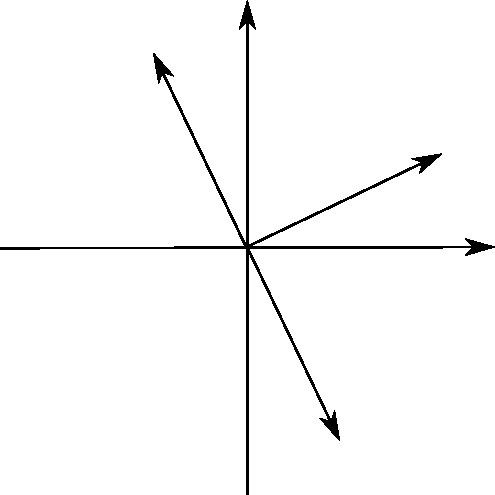
\includegraphics[width=0.6\textwidth]{Figures/VectorPhasesv2.pdf}};
\node at (155pt,270pt) {\Large{$y$}};
\node at (270pt,125pt) {\Large{$x$}};
\node at (60pt,230pt) {\Large{$\left(-v,u\right)$}};
\node at (220pt,205pt) {\Large{$\left(u,v\right)$}};
\node at (220pt,50pt) {\Large{$\left(v,-u\right)$}};
\end{tikzpicture}
\caption{The vector $(-v,u)$ is a phase $\pi/2$ ahead of the vector $(u,v)$, while the vector $(v,-u)$ is a phase $\pi/2$ behind the vector $(u,v)$.}
\label{fig:VectorPhases} 
\end{center}
\end{figure}
Using this, we find that the LLGS equations can be written as
\begin{subequations}
\begin{align}
    \nonumber&\left[-(i+\alpha\lambda_1)\omega - i\omega_0\lambda_1 - i\omega_J\lambda_2 -\frac{\omega_{\text{R}}}{1+\beta^2}P^{(y)}_1(i+\beta\lambda_1) + \omega^{(x)}_j\lambda_1(\lambda_2P^{(x)}_1 - P^{(x)}_0)\right]\tilde{\mathbold{u}}_1 \\
    + &\left[ i\omega_J\lambda_1 - \omega^{(x)}_jP^{(x)}_1 \right]\tilde{\mathbold{u}}_2 = 0, \\
    \nonumber&\left[i\omega_J\lambda_2 + \omega^{(x)}_jP^{(x)}_1\right]\tilde{\mathbold{u}}_1 \\
    + &\left[-(i+\alpha\lambda_2)\omega - i\omega_0\lambda_2 - i\omega_J\lambda_1 -\frac{\omega_{\text{R}}}{1+\beta^2}P^{(y)}_1(i+\beta\lambda_2) - \omega^{(x)}_j\lambda_1\lambda_2P^{(x)}_1 \right]\tilde{\mathbold{u}}_2 = 0.
\end{align}
\end{subequations}
Multiplying the equations above with $i$, we can write the equations compactly as
\begin{align}
    \label{eq:EigenvalueEqn_app}
    \left(\bar{A}\omega + \bar{V}\right)
    \begin{pmatrix}
     \tilde{\mathbold{u}}_1 \\
     \tilde{\mathbold{u}}_2
    \end{pmatrix}
    = 0,
\end{align}
with
\begin{subequations}
\begin{align}
    \bar{A} &=
    \begin{pmatrix}
     1-i\alpha\lambda_1 & 0 \\
     0 & 1-i\alpha\lambda_2
    \end{pmatrix}, \\
    \nonumber\bar{V} &=
    \omega_0\begin{pmatrix}
     \lambda_1 & 0 \\
     0 & \lambda_2
    \end{pmatrix}
    + \omega_J \begin{pmatrix}
     \lambda_2 & -\lambda_1 \\
     -\lambda_2 & \lambda_1
    \end{pmatrix}
    + i\omega_j^{(x)}\left[P_0
    \begin{pmatrix}
     -\lambda_1 & 0 \\
     0 & 0
    \end{pmatrix}
    + P_1
    \begin{pmatrix}
     \lambda_1\lambda_2 & -1 \\
     1 & -\lambda_1\lambda_2
    \end{pmatrix}\right] \\
    &\hspace{4.5mm} \frac{\omega_{\text{R}}^{(y)}}{1+\beta^2}\left[
    \begin{pmatrix}
     P_1^{(y)} & 0 \\
     0 & P_2^{(y)}
    \end{pmatrix}
    - i \beta
    \begin{pmatrix}
     P_1^{(y)}\lambda_1 & 0 \\
     0 & P_2^{(y)}\lambda_2
    \end{pmatrix}\right].
\end{align}
\end{subequations}

\section{Thin film geometry}
When considering the thin film geometry, there are four differences from the bulk geometry. Firstly, the easy axis is along $\mathbold{\hat{n}}_k = \mathbold{\hat{y}}$ instead of $\mathbold{\hat{n}}_k = \mathbold{\hat{z}}$. Secondly, the main inversion asymmetry is in the $z$-direction and there is only an applied current in the $x$-direction, so that the direction of the Rashba field becomes $\mathbold{\hat{z}}\times\mathbold{\hat{x}} = \mathbold{\hat{y}}$. For the bulk case this was also directed along $\mathbold{\hat{z}}$. Thirdly, as the easy axis is along $\mathbold{\hat{y}}$, we use the ansatz $\mathbold{m}_i = u^x_i\mathbold{\hat{x}}+\lambda_i\mathbold{\hat{y}}+u^z_i\mathbold{\hat{z}}$. Lastly, the polarizations in the Rashba field are given by the polarizations of the current in the $x$-direction, so that $\mathbold{H}^{\textrm{R}}_i \propto P^{(x)}_{i-1}$. With the exception of the last change, the difference between the thin film geometry and the bulk geometry is mainly a switch between the $y$- and $z$-directions. This makes it easier for us to find the matrices $\bar{A}$ and $\bar{V}$ for the thin film geometry. When switching two column vectors in a determinant you pick up a negative sign. When we switch the $y$- and $z$-directions, we therefore pick up a negative sign for the terms that stem from an odd number of cross products. Using this in addition to the fact that it is the current in the $x$-direction that generates the Rashba field, the equations for the thin film geometry can also be written in the form of \eqref{eq:EigenvalueEqn_app} with 
\begin{subequations}
\begin{align}
    \bar{A} &=
    \begin{pmatrix}
     1+i\alpha\lambda_1 & 0 \\
     0 & 1+i\alpha\lambda_2
    \end{pmatrix}, \\
    \nonumber\bar{V} &=
    -\omega_0\begin{pmatrix}
     \lambda_1 & 0 \\
     0 & \lambda_2
    \end{pmatrix}
    - \omega_J \begin{pmatrix}
     \lambda_2 & -\lambda_1 \\
     -\lambda_2 & \lambda_1
    \end{pmatrix}
    + i\omega_j^{(x)}\left[P_0
    \begin{pmatrix}
     -\lambda_1 & 0 \\
     0 & 0
    \end{pmatrix}
    + P_1
    \begin{pmatrix}
     \lambda_1\lambda_2 & -1 \\
     1 & -\lambda_1\lambda_2
    \end{pmatrix}\right] \\
    &\hspace{4.5mm} \frac{\omega_{\text{R}}^{(y)}}{1+\beta^2}\left[
    \begin{pmatrix}
     -P_0^{(x)} & 0 \\
     0 & P_1^{(x)}
    \end{pmatrix}
    - i \beta
    \begin{pmatrix}
     P_0^{(x)}\lambda_1 & 0 \\
     0 & P_1^{(x)}\lambda_2
    \end{pmatrix}\right].
\end{align}
\end{subequations}